\documentclass[10pt,aspectratio=43]{beamer}
\usepackage{tikz}
\usetheme{Boadilla}
\setbeamertemplate{navigation symbols}{}
\title{Cache invalidation: experiments and bounds}
\subtitle{Generated interaction study}
\author{Research group}
\date{}
\year=2026\month=11\day=5
\newcommand{\fuzzlayerA}[1]{\textbf{#1}}
\newcommand{\fuzzterm}[1]{\fuzzlayerA{#1}}
\newcommand{\fuzzpair}[2]{\fuzzterm{#1}: #2}
\newcommand{\fuzzunit}{ms}
\let\fuzzoriginalunit\fuzzunit
\newcommand{\fuzzcoefficient}{1}
\newcommand{\fuzzscale}[2][\fuzzcoefficient]{#1\,#2}
\definecolor{fuzzpaint}{RGB}{255,0,255}
\definecolor{fuzzsecond}{RGB}{18,137,67}
\tikzset{fuzzvertex/.style={draw,rounded corners=1pt,fill=blue!10,inner sep=1pt,minimum width=.35cm,minimum height=.25cm}}
\begin{document}
\section{Cache invalidation}
\begin{frame}[t,shrink=5]{Cache invalidation}{Composed dependencies}
\fuzzpair{Experiment}{Timing: 12\fuzzunit; estimate $\fuzzscale{x}+\fuzzscale[2]{y}$.}\par
{\renewcommand{\fuzzunit}{ticks}\let\fuzzterm\textrm\fuzzpair{LocalScope}{Timing: 7\fuzzunit.}\par}
\fuzzpair{RestoredScope}{Timing: 11\fuzzunit.}\par
\begin{columns}[onlytextwidth,b]
\begin{column}{0.46\textwidth}
\begin{columns}[onlytextwidth,c]
\begin{column}{0.54\textwidth}
{\small\color{teal}\centering
\textrm{A narrow column} can change line breaking even when the underlying expression is unchanged. The final diagram records the order in which information crosses the partition. The estimate is $\alpha+\beta$.\par}
\end{column}
\begin{column}{0.42\textwidth}
{\small\color{blue}\raggedleft
\begin{description}
\item[Stage 1] 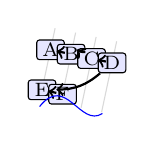
\begin{tikzpicture}[font=\scriptsize]
\begin{scope}[scale=0.8,rotate=-12]

\foreach \x in {0,1,2,3} {\draw[gray!30] (\x*0.333,-.8)--(\x*0.333,.35);}
\node[fuzzvertex] (g6n0) at (0.000,0) {A};
\node[fuzzvertex] (g6n1) at (0.333,0) {B};
\node[fuzzvertex] (g6n2) at (0.666,0) {C};
\node[fuzzvertex] (g6n3) at (0.999,0) {D};
\node[fuzzvertex] (g6n4) at (0.000,-0.65) {E};
\node[fuzzvertex] (g6n5) at (0.333,-0.65) {F};
\begin{scope}[xshift=.5pt,yshift=-.5pt]
\draw<1->[->,thick] (g6n0) -- (g6n1);
\draw<1->[->,thick] (g6n1) to[bend left=20] (g6n2);
\draw<1->[->,thick] (g6n2) -- (g6n3);
\draw<1->[->,thick] (g6n3) to[bend left=20] (g6n4);
\draw<1->[->,thick] (g6n4) -- (g6n5);
\draw[blue] (0,-.9) .. controls (0.300,-.3) and (0.699,-1.1) .. (0.999,-.8);
\end{scope}
\end{scope}
\end{tikzpicture}
\item[Stage 2] 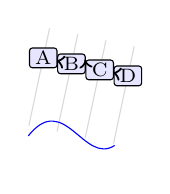
\begin{tikzpicture}[font=\scriptsize]
\begin{scope}[scale=1.1,rotate=-12]

\foreach \x in {0,1,2,3} {\draw[gray!30] (\x*0.333,-.8)--(\x*0.333,.35);}
\node[fuzzvertex] (g7n0) at (0.000,0) {A};
\node[fuzzvertex] (g7n1) at (0.333,0) {B};
\node[fuzzvertex] (g7n2) at (0.666,0) {C};
\node[fuzzvertex] (g7n3) at (0.999,0) {D};
\begin{scope}[xshift=.5pt,yshift=-.5pt]
\draw<1->[->,thick] (g7n0) -- (g7n1);
\draw<1->[->,thick] (g7n1) to[bend left=20] (g7n2);
\draw<1->[->,thick] (g7n2) -- (g7n3);
\draw[blue] (0,-.9) .. controls (0.300,-.3) and (0.699,-1.1) .. (0.999,-.8);
\end{scope}
\end{scope}
\end{tikzpicture}
\item[Stage 3] \textit{A local update} can change the measurements used by several neighboring components. The next pass must preserve the boundary conditions while revisiting dependent values. The estimate is $\frac{a+b}{1+c}$.
\end{description}\par}
\end{column}
\end{columns}
\end{column}
\begin{column}{0.50\textwidth}
\begin{columns}[onlytextwidth,c]
\begin{column}{0.38\textwidth}
{\small\color{blue}\raggedleft
\only<2->{\textit{The final diagram} records the order in which information crosses the partition.  The estimate is $\alpha+\beta$.}\par}
\end{column}
\begin{column}{0.58\textwidth}
\begin{alertblock}{Cache invalidation}
\begin{center}
\begin{tabular}{lrr}Method&Cost&Error\\\hline
Fresh0&8&11\\
Fresh1&13&27\\
Local2&18&1\\
Global3&17&29\\
\end{tabular}
\end{center}
\end{alertblock}
\end{column}
\end{columns}
\end{column}
\end{columns}
\par 
\begin{tikzpicture}[font=\scriptsize]
\fill<2-3>[fuzzpaint] (0,0) rectangle (.8,.3);
\fill<3->[fuzzsecond] (1,0) rectangle (1.8,.3);
\node[anchor=west] at (2,0.15) {Witness};
\end{tikzpicture}
\only<4>{}
\end{frame}
\renewcommand{\fuzzunit}{us}
\renewcommand{\fuzzcoefficient}{2}
\renewcommand{\fuzzterm}[1]{{\textbf{#1}}}
\section{Constraint propagation}
\begin{frame}[t]{Constraint propagation}
\fuzzpair{MacroStageB}{Timing: 12\fuzzunit, retained: 9\fuzzoriginalunit.}\par
{\renewcommand{\fuzzunit}{local}\fuzzpair{FrameLocal}{Timing: 5\fuzzunit.}\par}
\fuzzpair{FrameRestored}{Timing: 8\fuzzunit; estimate $\fuzzscale{x}$.}\par
\begin{columns}[T]\begin{column}{.46\textwidth}A local update can change the measurements used by several neighboring components.\end{column}\begin{column}{.46\textwidth}\begin{itemize}\item Input state\item Updated state\end{itemize}\end{column}\end{columns}
\end{frame}
\renewcommand{\fuzzunit}{Hz}
\renewcommand{\fuzzcoefficient}{3}
\renewcommand{\fuzzterm}[1]{{\textit{#1}}}
\section{Message passing}
\begin{frame}[t]{Incremental analysis}
\fuzzpair{MacroStageC}{Timing: 12\fuzzunit, retained: 9\fuzzoriginalunit.}\par
{\renewcommand{\fuzzunit}{local}\fuzzpair{FrameLocal}{Timing: 5\fuzzunit.}\par}
\fuzzpair{FrameRestored}{Timing: 8\fuzzunit; estimate $\fuzzscale{x}$.}\par
\begin{block}{Follow-up}\fuzzterm{A revised value} depends on the preceding frame.\end{block}
\[r_{k+1}=r_k-\alpha d_k\]
\end{frame}
\end{document}
